\documentclass{article}
\usepackage[utf8]{inputenc}
\usepackage[T1]{fontenc}
\usepackage[utf8]{inputenc}
\usepackage{lmodern}
\usepackage[a4paper, margin=1in]{geometry}
\usepackage{dirtree}
\usepackage{xcolor}
\usepackage{listings}
\usepackage{tabulary}
\usepackage{pdfpages}
\newcommand\myicon[1]{{\color{#1}\rule{2ex}{2ex}}}
\newcommand{\myfolder}[2]{\myicon{#1}\ {#2}}
\usepackage{minted}
\large
\title{C++ Assignment 1}

\setcounter{secnumdepth}{5}
\setcounter{tocdepth}{5}
\setlength{\parindent}{0em}
\setlength{\parskip}{1em}

\definecolor{codegreen}{rgb}{0,0.6,0}
\definecolor{codegray}{rgb}{0.5,0.5,0.5}
\definecolor{codepurple}{rgb}{0.58,0,0.82}
\definecolor{backcolour}{rgb}{0.95,0.95,0.92}

\lstdefinestyle{mystyle}{
    backgroundcolor=\color{backcolour},   
    commentstyle=\color{codegreen},
    keywordstyle=\color{magenta},
    numberstyle=\tiny\color{codegray},
    stringstyle=\color{codepurple},
    basicstyle=\ttfamily\footnotesize,
    breakatwhitespace=false,         
    breaklines=true,                 
    captionpos=b,                    
    keepspaces=true,                 
    numbers=left,                    
    numbersep=5pt,                  
    showspaces=false,                
    showstringspaces=false,
    showtabs=false,                  
    tabsize=2
}

\lstset{style=mystyle}

\begin{document}
\begin{titlepage}
	\begin{center}
    \line(1,0){300}\\
    [0.65cm]
	\huge{\bfseries ICT374 - Assignment II}\\
	\line(1,0){300}\\
	\textsc{\Large FTP Server and Client}\\
	\textsc{\LARGE \today}\\
	[5.5cm]     
	\end{center}
	\begin{flushright}
		\textsc{\Large Kiera Gibson\\33582181}\\
		[0.5cm]
		\textsc{\Large Peter S. Crabbe\\32019269}\\
		[0.5cm]
	\end{flushright}
\end{titlepage}

\tableofcontents
\section{Project Declaration}
\includepdf[pages=-]{ICT374ProjectDeclaration}
\newpage
\section{List of Files}
\dirtree{%
.1 \myfolder{red}{Assignment 2}.
.2 \myfolder{blue}{client}.
.3 \myfolder{green}{client.h}.
.3 \myfolder{green}{client.c}.
.3 \myfolder{green}{main.h}.
.3 \myfolder{green}{main.c}.
.2 \myfolder{blue}{server}.
.3 \myfolder{green}{main.h}.
.3 \myfolder{green}{main.c}.
.2 \myfolder{blue}{shared}.
.3 \myfolder{green}{include}.
.4 \myfolder{orange}{shared.h}.
.4 \myfolder{orange}{token.h}.
.4 \myfolder{orange}{directory\_handling.h}.
.3 \myfolder{green}{src}.
.4 \myfolder{orange}{shared.c}.
.4 \myfolder{orange}{token.c}.
.4 \myfolder{orange}{directory\_handling.c}.
.2 \myfolder{blue}{lib}.
.3 \myfolder{green}{json-c}.
.3 \myfolder{green}{base64}.
.2 \myfolder{blue}{documentation}.
.3 \myfolder{green}{Assignment2.tex}.
}

\section{PreInformation}
Extension from the Unit Coordinator was given and is attached below. \\
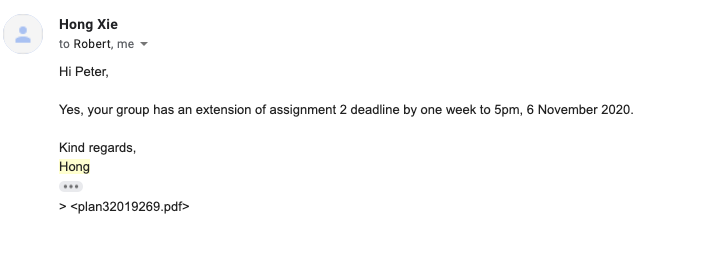
\includegraphics[width=\textwidth]{extension}

The group also asked permission to use CMake to generate the Make file. Hong Advised as long as it can make a make file and build using make this was acceptable. The guide on how to use Cmake is in the Building section.\\
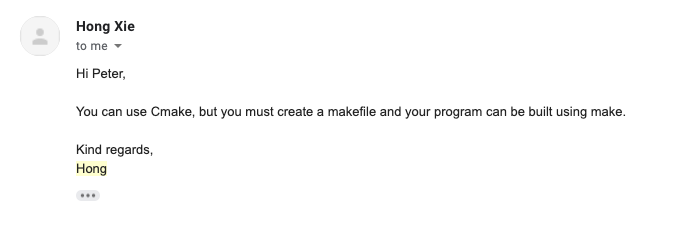
\includegraphics[width=\textwidth]{make}

The group also asked that we be able to use JSON for our messaging. This allowed us to simplify our string parsing. Permission was granted. This also meant we needed to use an encoder for binary data as any null terminators would break our JSON stream. Attached is the email approving this.\\
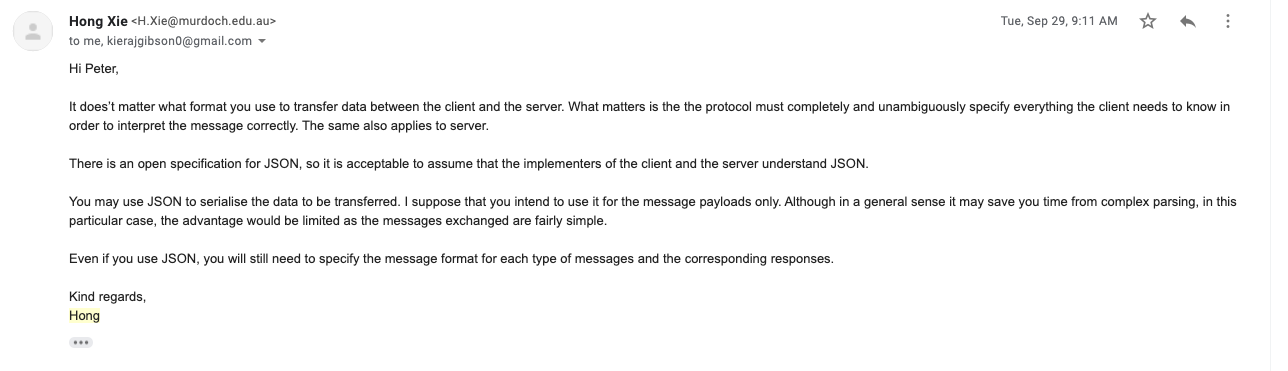
\includegraphics[width=\textwidth]{json}

\section{Information}
Design and implement a simple network protocol that can be used to download files from a remote site and to upload files to a remote site, and a client and a server programs that communicate using that protocol. The protocol is using TCP as its transport layer protocol. The server can have multiple clients request simultaneously. For simplicity we did not consider any authentication process in this project, hence the server will provide its service to any client with the right site address and port number.

\section{Self Diagnosis and Evaluation}
\subsection{Working}
\begin{itemize}
\item The way we have implemented our code makes it portable while also being cross platform on both macOS to Linux. This does make it more complicated and with out extensive checking possibly more error prone.
\item Using a shared library between our client and our server gives us the ability to keep shared code consistent between both the server and client. This avoids any issues of changes to one causing unpredictable behaviour in the other.
\item Using a third party library for serialisation and deserialisation means that our backbone is robust and simpler to parse. This removes any headaches that come with parsing strings in C.
\item All functions that are required are implemented and working. This includes PUT, GET, CD, LCD, DIR, LDIR, PWD, LPWD and QUIT.
\item PUT and GET work with both text and binary data.
\item The server is able to work across the internet and has been tested with multiple clients connecting at the same time with no issues.
\end{itemize}

\subsection{Not Working}
\begin{itemize}
    \item While the program can reap child processes, Due to the socket blocking it wont be able to end our connection while loop until another client attempts to connect. Releasing the block and allowing the program to reap its children. Had we more time this could have been easily been fixed.
    \item Both Put and Get will not work from files from different folders that are not in the current working directory. This is due to the way we handle the transfer of data.
\end{itemize}

\section{Solution Breakdown}
The solution devised is that there is a client and a server program. However, a large chunk of code is required in both. We needed to ensure that the client and the server followed the protocols and any under the hood changes to one side didn't break the other. This was solved by having our own shared library that both programs pull down from. By doing this way, refactoring chunks of code can be achieved with out breaking the functions calling them.\\

The underlying data structure for communication from client and server is JSON. This allows us to use key data pairs. If a key exists the data corresponding to the key must exist. This ensures that parsing data is simple, safe and effective. The reason this is safer is because we are able to stop a function if a key is missing and instead report and error.\\

A short fall in using JSON is that any string must only be null terminated once. This means that binary data is dangerous being stored in a json string. To ensure avoiding this limitation, we encode our data into base64. While this can give us a 40\% overhead on file size at the absolute worst, this ensures that the JSON payload wont break during transmission. We believe that the trade off is worth the reliability that JSON offers.

\section{Protocol}
\subsection{Commands and JSON}
As mentioned prior, JSON is the backbone of the FTP client and server as it allows for serialisation and deserialisation of the data between the two. Another benefit of implementing JSON is that if an error occurs in this process we can also assume that the data sent was not completed.

Each bolded word in a dot point is a key value in the JSON.

\subsubsection{CD}
Changes the current directory on the server.

Client Sends.
\begin{itemize}
\item \textbf{command:} The command to be processed on the server.
\item \textbf{dir:} The directory to be changed into relative to the current directory. 
\end{itemize}

Server Response.
\begin{itemize}
\item \textbf{error:} The error number reported by the operation of the function. 0 represents no error.   
\end{itemize}

\subsubsection{DIR}
Lists all the the directories and file relative the current working directory on the server.

Client Sends.
\begin{itemize}
\item \textbf{command:} The command to be processed on the server.
\end{itemize}

Server Response.
\begin{itemize}
\item \textbf{directoryError:} An error if the directory fails to open accordingly.
\item \textbf{scandirError:} The error produced if the scan in the directory for files and folders fails. Anything above or equal to 0 is an error.
\item \textbf{arraySize:} The size of the array of directories.
\item \textbf{array:} The array of strings for each file / folder that is in the current working directory of the server.
\item \textbf{currentDirectory:} The current working directory of the server so the client knows the location of the output given.
\end{itemize}

\subsubsection{PWD}
Gives the absolute path to the current working directory of the server.

Client Sends
\begin{itemize}
\item \textbf{command:} The command to be processed on the server.
\end{itemize}

Server Response
\begin{itemize}
\item \textbf{cwd:} The current working directory of the server.
\item \textbf{error:} The error number reported by the operation of the function. 0 represents no error.
\end{itemize}

\subsubsection{PUT}
Takes a file from the client and places it on the server.

Client Sends.
\begin{itemize}
\item \textbf{command:} The command to be processed on the server.
\item \textbf{filename:} The file name to write the data too.
\item \textbf{filedata:} Data of the file that was sent, this is encoded in base64 to ensure that null terminators do not break the json string.
\item \textbf{ensize:} The encoded length of the string.
\item \textbf{desize:} The decoded length of the string.
\end{itemize}

Server Response.
\begin{itemize}
\item \textbf{error:} The error number reported by the operation of the function. 0 represents no error.
\end{itemize}

\subsubsection{GET}
Takes a file from the server and places it on the client.

Client Sends.
\begin{itemize}
\item \textbf{command:} The command to be processed on the server.
\end{itemize}

Server Reponse.
\begin{itemize}
\item \textbf{filename:} The file name to write the data too.
\item \textbf{filedata:} Data of the file that was sent, this is encoded in base64 to ensure that null terminators do not break the json string.
\item \textbf{ensize:} The encoded length of the string.
\item \textbf{desize:} The decoded length of the string.
\item \textbf{error:} The error number reported by the operation of the function. 0 represents no error.
\end{itemize}

\subsection{Send and Receive}
The functions listed above all use the existing TCP protocol implemented by the POSIX standards.
\subsubsection{Send Protocol}
The send protocol that is implemented following these rules. The protocol sends only JSON objects that have been deserialised.
\begin{enumerate}
    \item Attempt to send the size of the data the recipient needs to receive.
    \item Await a response to confirm the recipient is ready. If no value or a false value is received, terminate send.
    \item Recipient sends confirmation that it is ready.
    \item Send payload, deduct how many bytes were sent from the total until the total is equal to zero.
    \item Return 0 if success otherwise return -1.
\end{enumerate}
\subsubsection{Receive Protocol}
The receive protocol that is implemented following these rules. The protocol receives only JSON objects that have been deserialised. Once the final step is complete it is then serialised back into JSON to be parsed.
\begin{enumerate}
    \item Wait for sender to confirm the size of the data.
    \item If size is received acknowledge by sending true, else send false and terminate receive process.
    \item Await sender to begin transfer of data.
    \item Keep looping until the current size is equal to agreed upon size.
    \item If receive error, terminate; else update buffer parameter and return the size to the buffer.
\end{enumerate}
\section{Building}
\subsection{Dependencies}
\subsubsection*{Linux}
The following dependencies are required for Linux.
\begin{itemize}
    \item Cmake 3.14
    \item gcc or clang compiler
\end{itemize}
\begin{lstlisting}
        sudo apt install cmake
\end{lstlisting}
\subsubsection*{macOS}
\begin{itemize}
    \item Cmake 3.14
    \item Brew
    \item gcc or clang compiler
\end{itemize}
\begin{lstlisting}
        brew install cmake
\end{lstlisting}
\subsection{Building}
\begin{center}
\textbf{Please ensure you have the dependencies before you continue.}
\end{center}
To generate the build scripts please run from the root directory....
\begin{lstlisting}
cmake -S . -B build -D CMAKE_BUILD_TYPE=Release    
\end{lstlisting}
Change into the build directory
\begin{lstlisting}
cd build/    
\end{lstlisting}
Now call make to begin the compilation process like so.
\begin{lstlisting}
make myftp myftpd    
\end{lstlisting}
The compiler should have produced 2 unix executables, myftp is the client program and myftpd is the server program. Below is the build output of the make file that was compiled with "-Wall -Wextra" flags showing the program compiles with no warnings or errors. The program was also ran using Valgrind to find and fix any memory leaks. 

\begin{lstlisting}
Scanning dependencies of target base64
[  1%] Building C object lib/base64/CMakeFiles/base64.dir/lib/arch/avx2/codec.c.o
[  3%] Building C object lib/base64/CMakeFiles/base64.dir/lib/arch/generic/codec.c.o
[  5%] Building C object lib/base64/CMakeFiles/base64.dir/lib/arch/neon32/codec.c.o
[  7%] Building C object lib/base64/CMakeFiles/base64.dir/lib/arch/neon64/codec.c.o
[  9%] Building C object lib/base64/CMakeFiles/base64.dir/lib/arch/ssse3/codec.c.o
[ 11%] Building C object lib/base64/CMakeFiles/base64.dir/lib/arch/sse41/codec.c.o
[ 13%] Building C object lib/base64/CMakeFiles/base64.dir/lib/arch/sse42/codec.c.o
[ 15%] Building C object lib/base64/CMakeFiles/base64.dir/lib/arch/avx/codec.c.o
[ 17%] Building C object lib/base64/CMakeFiles/base64.dir/lib/lib.c.o
[ 19%] Building C object lib/base64/CMakeFiles/base64.dir/lib/codec_choose.c.o
[ 21%] Building C object lib/base64/CMakeFiles/base64.dir/lib/tables/tables.c.o
[ 23%] Linking C static library libbase64.a
[ 23%] Built target base64
Scanning dependencies of target json-c
[ 25%] Building C object lib/json-c/CMakeFiles/json-c.dir/arraylist.c.o
[ 27%] Building C object lib/json-c/CMakeFiles/json-c.dir/debug.c.o
[ 29%] Building C object lib/json-c/CMakeFiles/json-c.dir/json_c_version.c.o
[ 31%] Building C object lib/json-c/CMakeFiles/json-c.dir/json_object.c.o
[ 33%] Building C object lib/json-c/CMakeFiles/json-c.dir/json_object_iterator.c.o
[ 35%] Building C object lib/json-c/CMakeFiles/json-c.dir/json_pointer.c.o
[ 37%] Building C object lib/json-c/CMakeFiles/json-c.dir/json_tokener.c.o
[ 39%] Building C object lib/json-c/CMakeFiles/json-c.dir/json_util.c.o
[ 41%] Building C object lib/json-c/CMakeFiles/json-c.dir/json_visit.c.o
[ 43%] Building C object lib/json-c/CMakeFiles/json-c.dir/linkhash.c.o
[ 45%] Building C object lib/json-c/CMakeFiles/json-c.dir/printbuf.c.o
[ 47%] Building C object lib/json-c/CMakeFiles/json-c.dir/random_seed.c.o
[ 49%] Building C object lib/json-c/CMakeFiles/json-c.dir/strerror_override.c.o
[ 50%] Linking C shared library libjson-c.dylib
[ 50%] Built target json-c
Scanning dependencies of target myftp-shared
[ 52%] Building C object shared/CMakeFiles/myftp-shared.dir/src/shared.c.o
[ 54%] Building C object shared/CMakeFiles/myftp-shared.dir/src/token.c.o
[ 56%] Building C object shared/CMakeFiles/myftp-shared.dir/src/directory_handling.c.o
[ 58%] Linking C static library libmyftp-shared.a
[ 58%] Built target myftp-shared
Scanning dependencies of target myftp
[ 60%] Building C object CMakeFiles/myftp.dir/client/main.c.o
[ 62%] Building C object CMakeFiles/myftp.dir/client/client.c.o
[ 64%] Linking C executable myftp
[ 64%] Built target myftp
Scanning dependencies of target myftpd
[ 66%] Building C object CMakeFiles/myftpd.dir/server/main.c.o
[ 68%] Linking C executable myftpd
[ 68%] Built target myftpd
Scanning dependencies of target json-c-static
[ 70%] Building C object lib/json-c/CMakeFiles/json-c-static.dir/arraylist.c.o
[ 72%] Building C object lib/json-c/CMakeFiles/json-c-static.dir/debug.c.o
[ 74%] Building C object lib/json-c/CMakeFiles/json-c-static.dir/json_c_version.c.o
[ 76%] Building C object lib/json-c/CMakeFiles/json-c-static.dir/json_object.c.o
[ 78%] Building C object lib/json-c/CMakeFiles/json-c-static.dir/json_object_iterator.c.o
[ 80%] Building C object lib/json-c/CMakeFiles/json-c-static.dir/json_pointer.c.o
[ 82%] Building C object lib/json-c/CMakeFiles/json-c-static.dir/json_tokener.c.o
[ 84%] Building C object lib/json-c/CMakeFiles/json-c-static.dir/json_util.c.o
[ 86%] Building C object lib/json-c/CMakeFiles/json-c-static.dir/json_visit.c.o
[ 88%] Building C object lib/json-c/CMakeFiles/json-c-static.dir/linkhash.c.o
[ 90%] Building C object lib/json-c/CMakeFiles/json-c-static.dir/printbuf.c.o
[ 92%] Building C object lib/json-c/CMakeFiles/json-c-static.dir/random_seed.c.o
[ 94%] Building C object lib/json-c/CMakeFiles/json-c-static.dir/strerror_override.c.o
[ 96%] Linking C static library libjson-c.a
[ 96%] Built target json-c-static
Scanning dependencies of target json_parse
[ 98%] Building C object lib/json-c/apps/CMakeFiles/json_parse.dir/json_parse.c.o
[100%] Linking C executable ../../../json_parse
[100%] Built target json_parse    
\end{lstlisting}


\section{Executing}
\subsection{Server}
To run the server just execute myftpd, no additional information is required.
\begin{lstlisting}
    ./myftpd
\end{lstlisting}
\subsection{Client}
Running the client, an IP address will need to be parsed in should you wish to connect to a server that is not local. Failing to provide an IP address on the first argument will result in the IP being bound to 127.0.0.1. 

Example of setting an ip...
\begin{lstlisting}
    ./myftp 1.1.1.1
\end{lstlisting}
or
\begin{lstlisting}
    ./myftp arkwolf.com
\end{lstlisting}


\section{Test Evidence}
\subsection{User Testing}
%
%\textbf{Task:} \\
%\textbf{Action:} \\
%\textbf{Result:} \\

\textbf{Task:} Execute Client\\
\textbf{Action:} User input into shell "./myftp"\\
\textbf{Result:} Was able to connect to the local myftpd server when the server was running on my local machine.\\
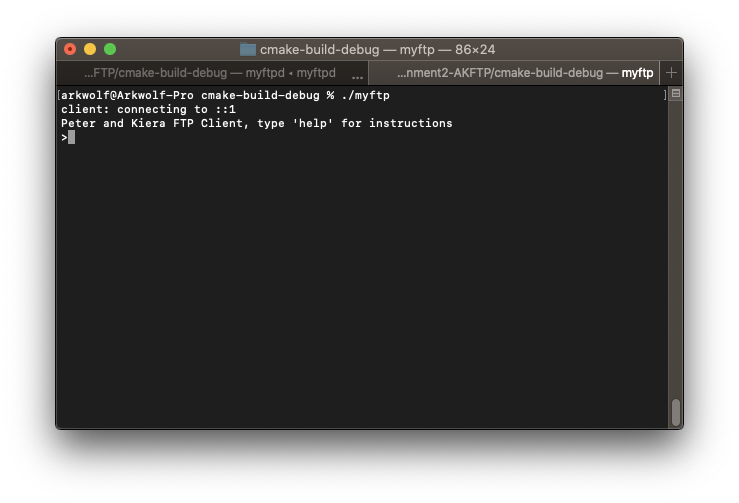
\includegraphics[width=\textwidth]{testpictures/connect}

\textbf{Task:} Execute Client with DNS\\
\textbf{Action:} User Input into shell "./myftp arkwolf.com"\\
\textbf{Result:} Was able to connect to the remote server myftpd server when the server was running on my remote machine.\\
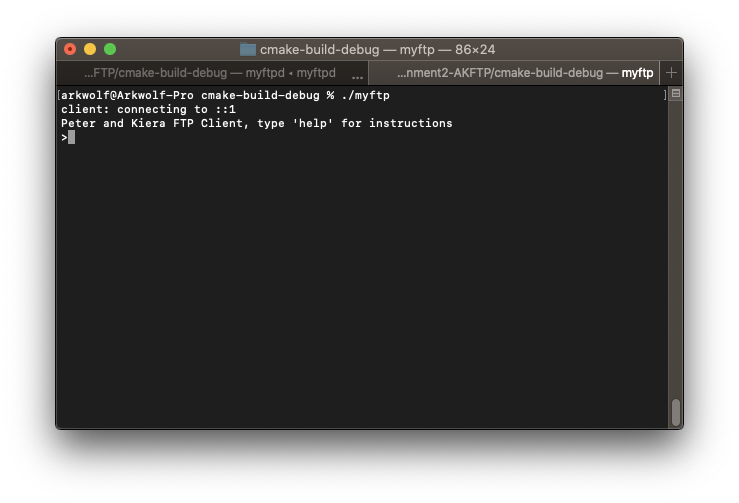
\includegraphics[width=\textwidth]{testpictures/connect}

\textbf{Task:} Test the pwd command to the server.\\
\textbf{Action:} pwd\\
\textbf{Result:} The server returned its current working directory and performed as expected. Output: /Users/arkwolf/Documents/Coding Schoolwork/ICT374-Assignment2-AKFTP/cmake-build-debug/final/server\\
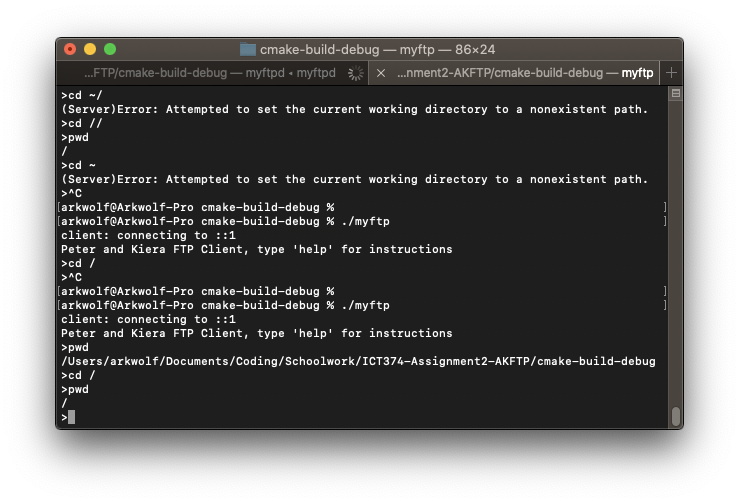
\includegraphics[width=\textwidth]{testpictures/pwd}

\textbf{Task:} Test the lpwd command to the client.\\
\textbf{Action:} lpwd\\
\textbf{Result:} The client returned its current working directory and performed as expected. Output: /Users/arkwolf/cuments/Coding/Schoolwork/ICT374-Assignment2-AKFTP/cmake-build-debug/final/client\\
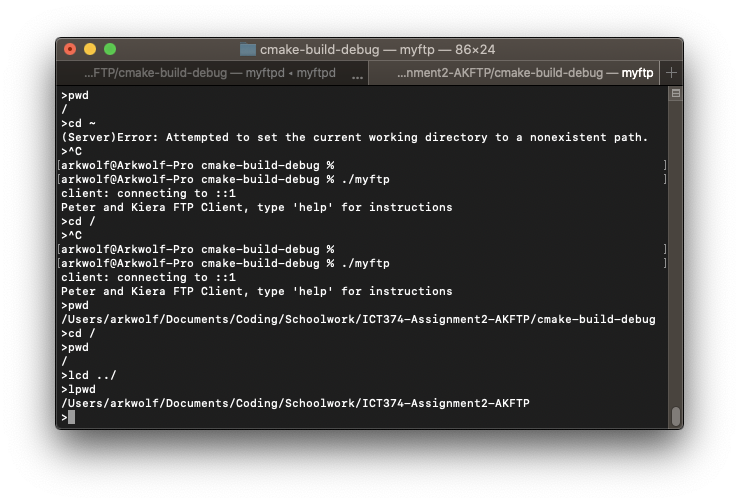
\includegraphics[width=\textwidth]{testpictures/lpwd}

\textbf{Task:} Change the directory using the CD command.\\
\textbf{Action:} cd ../\\
\textbf{Result:} No output, indicating a success.\\
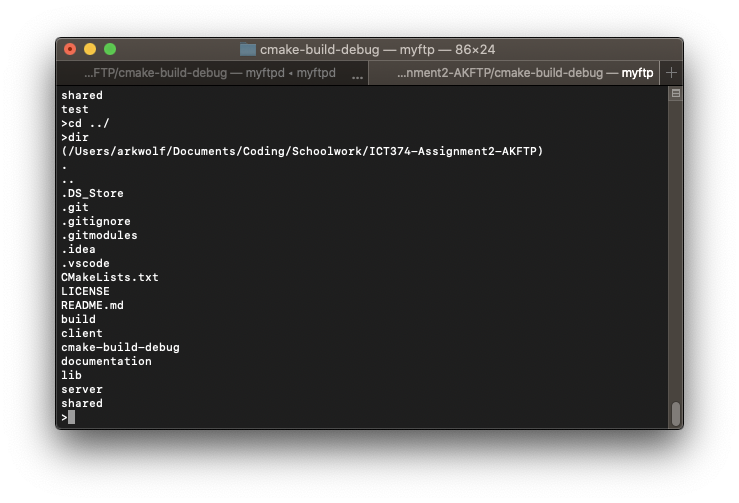
\includegraphics[width=\textwidth]{testpictures/cdserver}

\textbf{Task:} Change the directory using the local cd command\\
\textbf{Action:} lcd ../\\
\textbf{Result:} No output, indicating a success.\\
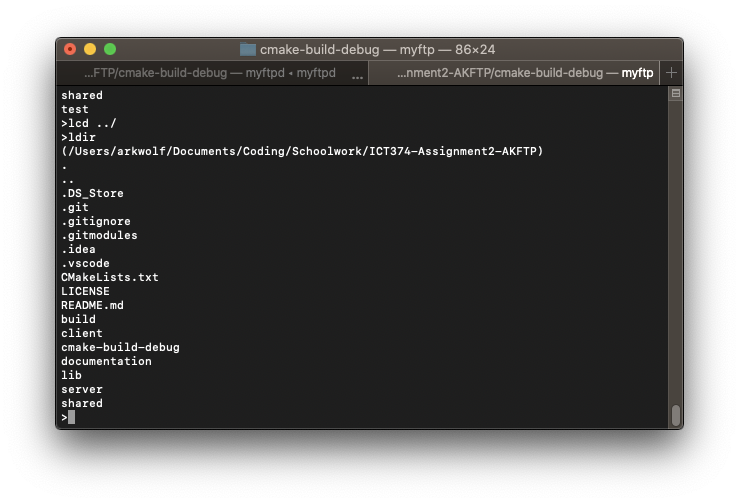
\includegraphics[width=\textwidth]{testpictures/lcd}

\textbf{Task:} Get a list of the directories inside the servers current working directory.\\
\textbf{Action:} dir\\
\textbf{Result:} The server returned a list of its folders and files at its current working directory as expected.\\
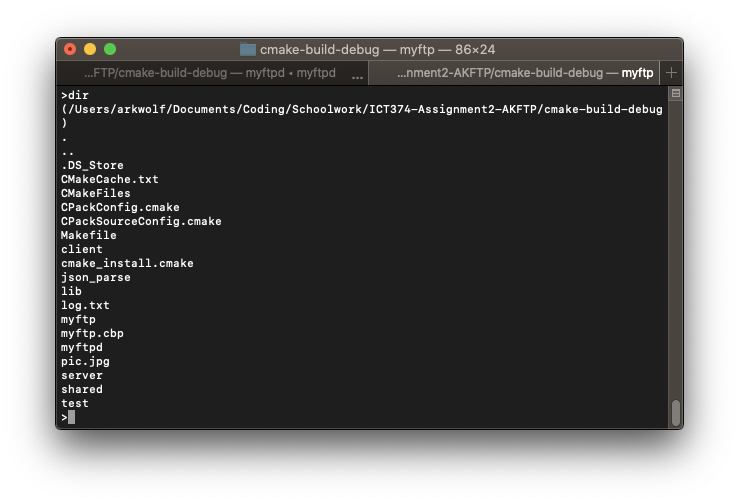
\includegraphics[width=\textwidth]{testpictures/dir}

\textbf{Task:} Get a list of the directories inside the clients current working directory.\\\
\textbf{Action:} ldir\\
\textbf{Result:} The client returned a list of its folders and files at its current working directory as expected.\\
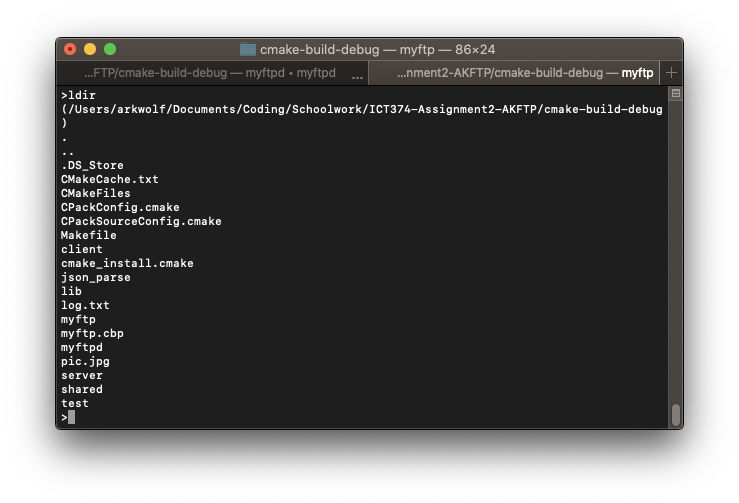
\includegraphics[width=\textwidth]{testpictures/ldir}

\textbf{Task:} Upload a text file.\\
\textbf{Action:} put touch.txt\\
\textbf{Result:} The text file from the clients working directory was uploaded to the servers local directory.\\
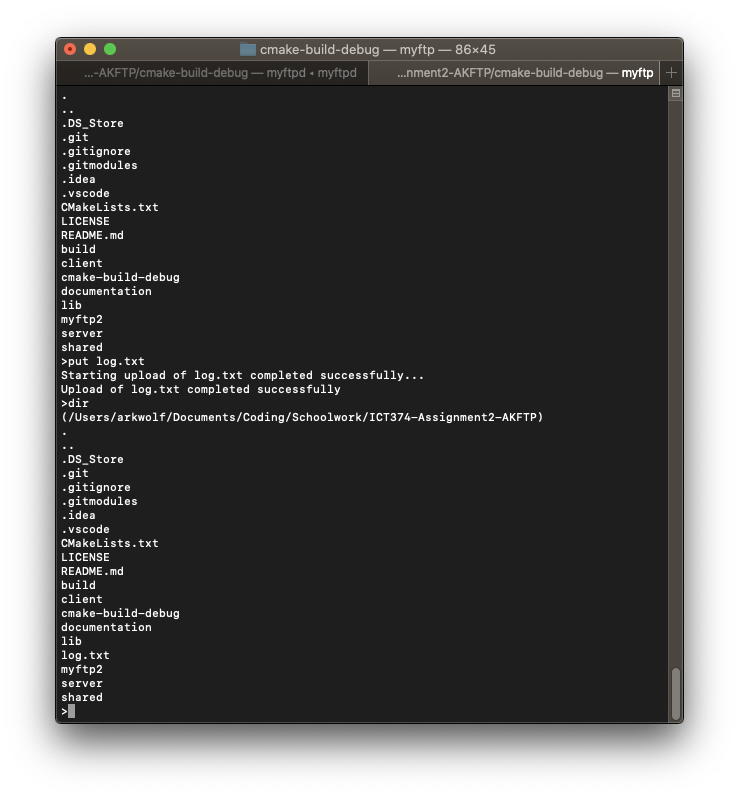
\includegraphics[width=\textwidth]{testpictures/puttext}

\textbf{Task:} Upload a binary file\\
\textbf{Action:} put myftpd\\
\textbf{Result:} The binary file from the clients working directory was uploaded to the servers local directory.\\
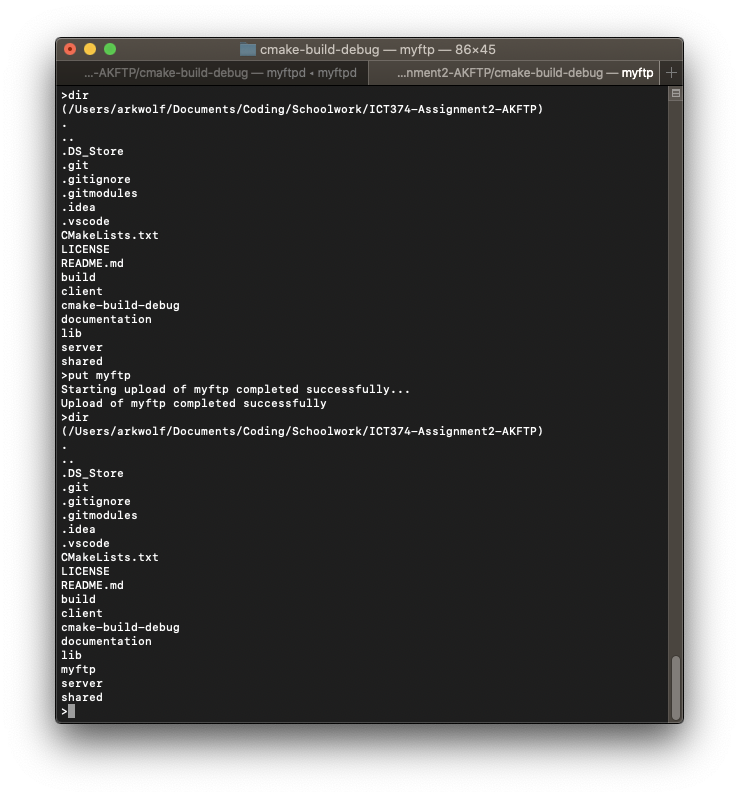
\includegraphics[width=\textwidth]{testpictures/putbinary}

\textbf{Task:} Download a text file\\
\textbf{Action:} get touch.txt\\
\textbf{Result:} The text file from the servers working directory was downloaded to the clients local directory.\\
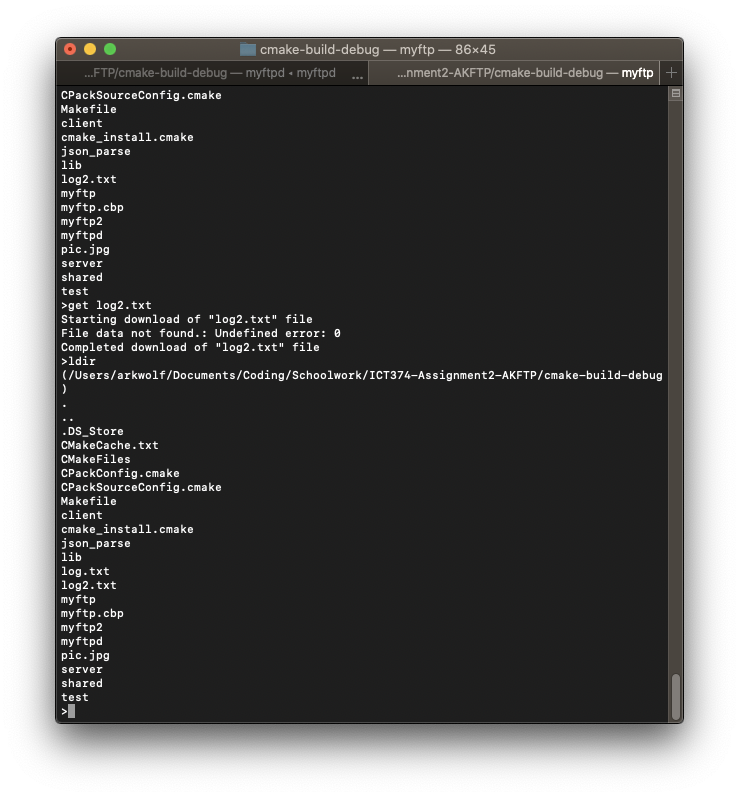
\includegraphics[width=\textwidth]{testpictures/gettext}

\textbf{Task:} Download a binary file\\
\textbf{Action:} get myftpd\\
\textbf{Result:} The binary file from the servers working directory was downloaded to the clients local directory.\\
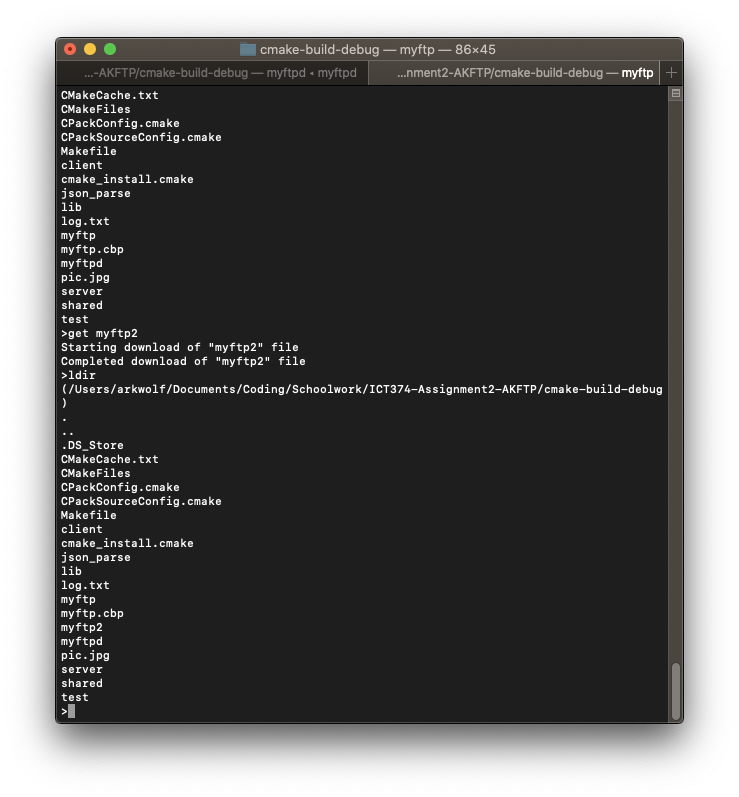
\includegraphics[width=\textwidth]{testpictures/getbinary}

\textbf{Task:} Download a file with spaces\\
\textbf{Action:} get "space pic.jpg"\\
\textbf{Result:} The binary file with spaces in the filename from the servers working directory was downloaded to the clients local directory.\\
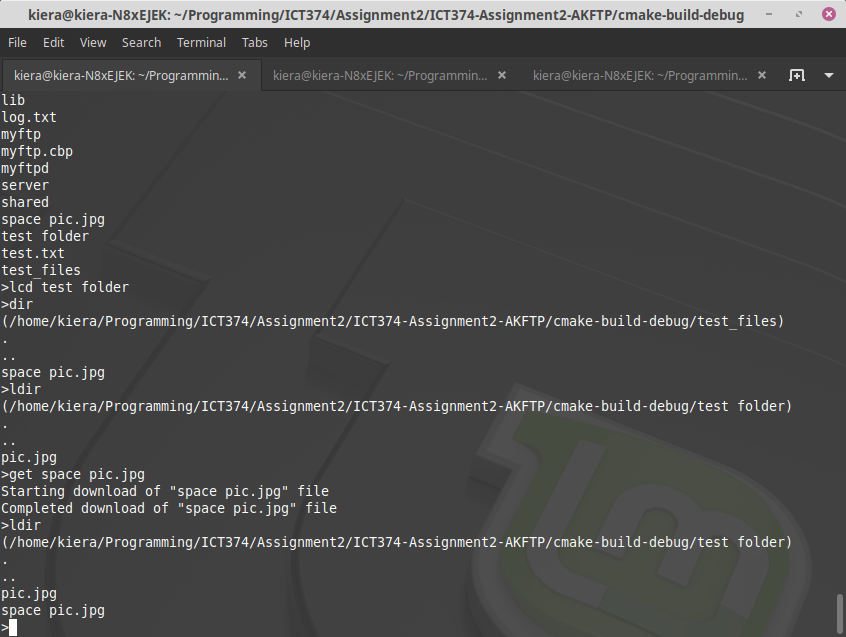
\includegraphics[width=\textwidth]{testpictures/space_get}

\textbf{Task:} Upload a file with spaces\\
\textbf{Action:} put "space pic.jpg"\\
\textbf{Result:} The binary file with spaces in the filename from the clients working directory was uploaded to the servers local directory.\\
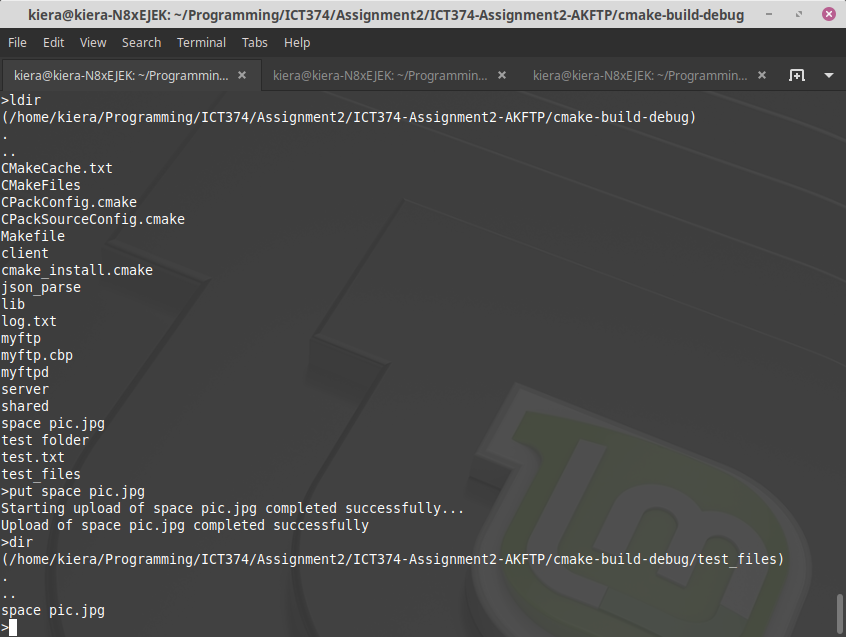
\includegraphics[width=\textwidth]{testpictures/space_put}


\newpage
\section{Source Code Listing}
\subsection{Client}
    \subsubsection{main.c}
	\lstinputlisting[language=C]{../client/main.c}
	\subsubsection{client.c}
	\lstinputlisting[language=C]{../client/client.c}
\subsection{Server}
    \subsubsection{main.c}
	\lstinputlisting[language=C]{../server/main.c}
\subsection{Shared}
    \subsubsection{shared.c}
	\lstinputlisting[language=C]{../shared/src/shared.c}
	\subsubsection{token.c}
	\lstinputlisting[language=C]{../shared/src/token.c}
	\subsubsection{directory\_handling.c}
	\lstinputlisting[language=C]{../shared/src/directory_handling.c}

\section{Third-Party Source Code}
\subsection{json-c}
JSON library used under MIT license.\\
Thank you to all the contributors.\\
https://github.com/json-c/json-c/\\
\subsection{base64}
Base 64 encorder used to encode and decode our data streams.\\
Licensed under BSD-Clause "Simplified" License.\\
Thank you to all the contributors.\\
https://github.com/aklomp/base64\\
\end{document}